% =============================================================================
% PART A (CONTINUED): PORT MAPPING, DOCKER COMPOSE, LOCAL DEV & VERIFICATION
% Project: Frevia - AI-Powered Freelance Marketplace & Community Platform
% In Charge: Nguyen Tien Thuan (CE181024)
% =============================================================================

\subsection{Service Port Mapping}

When operating the complete system on a local host or cloud virtual machine, the \textbf{Frevia} architecture utilizes the following default network ports. The system administrator or developer must verify that these ports are unoccupied prior to starting the containers:

\begin{center}
\renewcommand{\arraystretch}{1.45}
\begin{tabular}{|L{3.2cm}|L{3.2cm}|C{2.0cm}|L{5.6cm}|}
\hline
\rowcolor{hdrfill}\hd{Service Name} & \hd{Container Name} & \hd{Port} & \hd{Endpoint URL \& Functional Role} \\ \hline
\textbf{Frontend Web} & \texttt{frevia-web} & \texttt{3001} & \url{http://localhost:3001} -- Next.js 16 Client Portal and Admin Management Console. \\ \hline
\textbf{Backend API} & \texttt{frevia-api} & \texttt{3000} & \url{http://localhost:3000} -- NestJS 11 RESTful API endpoints and WebSocket gateway. \\ \hline
\textbf{PostgreSQL DB} & \texttt{frevia-postgres} & \texttt{5432} & \texttt{localhost:5432} -- Primary relational database storage (Database: \texttt{frevia}). \\ \hline
\textbf{Redis Server} & \texttt{frevia-redis} & \texttt{6379} & \texttt{localhost:6379} -- In-memory caching engine, OTP storage, and session broker. \\ \hline
\textbf{pgAdmin 4} & \texttt{frevia-pgadmin} & \texttt{5050} & \url{http://localhost:5050} -- Web-based database management and visualization console. \\ \hline
\end{tabular}
\end{center}

\subsection{System Startup Options}

The platform supports \textbf{two distinct execution workflows} tailored for production-like evaluation and daily development:

\subsubsection{Option 1: Automated Deployment via Docker Compose (Recommended)}

This workflow packages and orchestrates all 5 system services (\texttt{postgres}, \texttt{redis}, \texttt{pgadmin}, \texttt{api}, \texttt{web}) within an isolated internal bridge network (\texttt{frevia-network}) using a single terminal command:

\begin{figure}[H]
  \centering
  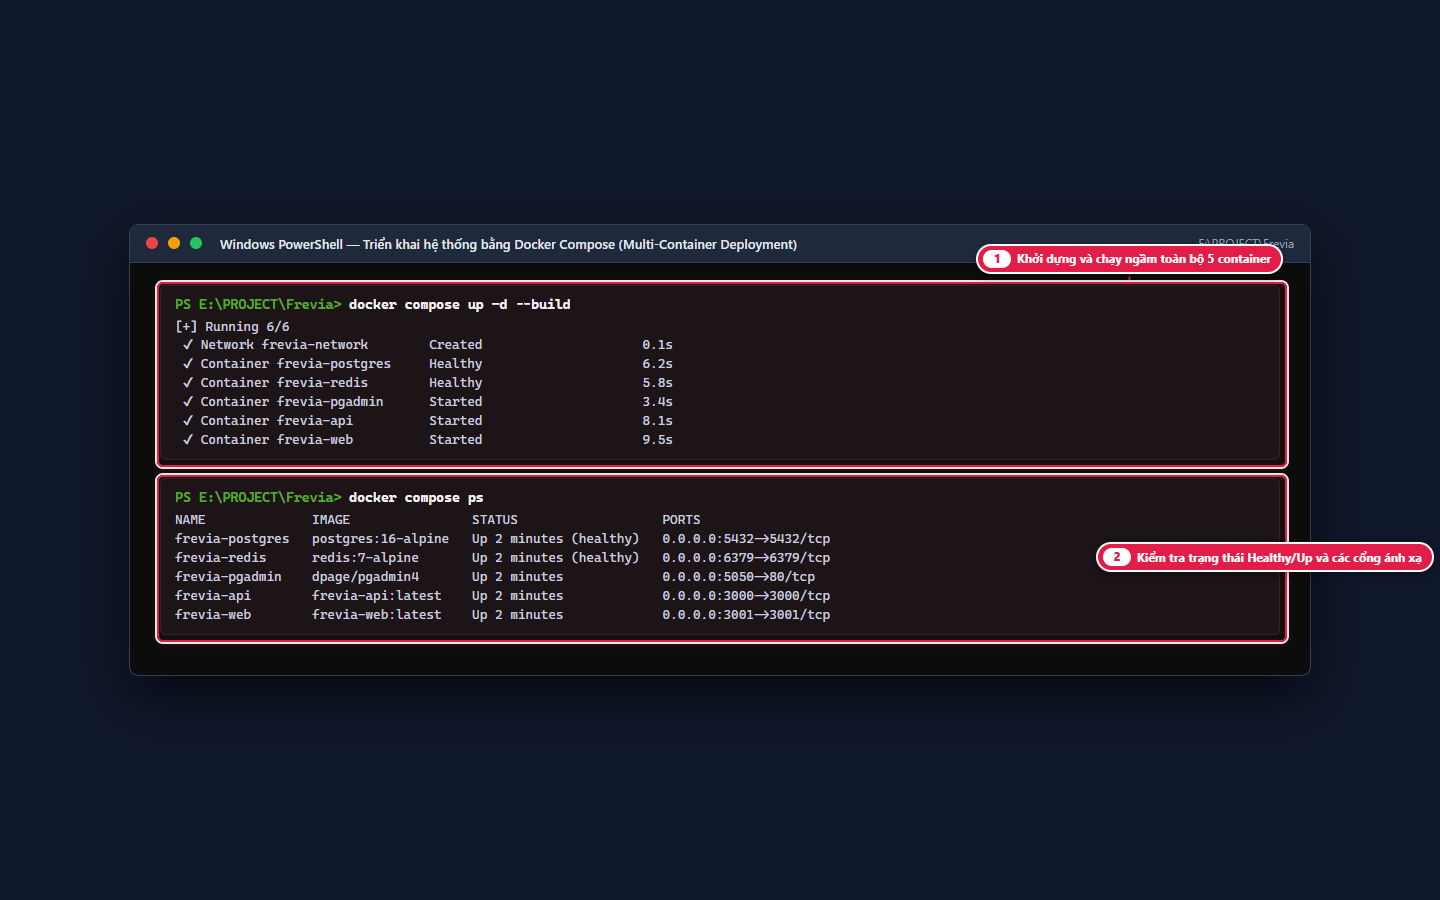
\includegraphics[width=0.90\textwidth]{images/install/a08_docker_compose_up.png}
  \caption{Building and deploying all 5 system containers using Docker Compose}
\end{figure}

\begin{itemize}[leftmargin=1.5em,itemsep=3pt]
  \item \rbadge{1} In the root directory of the repository, execute:
\begin{lstlisting}[frame=single,basicstyle=\footnotesize\ttfamily,backgroundcolor=\color{codebg}]
docker compose up -d --build
\end{lstlisting}
  Docker builds production images for the API and Web applications, initializes persistent volumes, and launches all containers in detached mode.
  \item \rbadge{2} Run \texttt{docker compose ps} to verify container execution states: confirm that the database and cache report \texttt{Up (healthy)} status and the port mappings align with the architecture specification.
  \item Routine monitoring and shutdown commands:
\begin{lstlisting}[frame=single,basicstyle=\footnotesize\ttfamily,backgroundcolor=\color{codebg}]
# Tail live logs for the API and Web services
docker compose logs -f api web

# Gracefully terminate all containers while retaining database volume data
docker compose down
\end{lstlisting}
\end{itemize}

\subsubsection{Option 2: Local Development Workflow}

For active development with hot-module reloading and interactive debugging:
\begin{enumerate}[leftmargin=1.8em,itemsep=3pt]
  \item Start the backend infrastructure services via Docker:
\begin{lstlisting}[frame=single,basicstyle=\footnotesize\ttfamily,backgroundcolor=\color{codebg}]
docker compose up -d postgres redis pgadmin
\end{lstlisting}
  \item Launch the NestJS backend and Next.js frontend concurrently across the monorepo:
\begin{lstlisting}[frame=single,basicstyle=\footnotesize\ttfamily,backgroundcolor=\color{codebg}]
pnpm dev
\end{lstlisting}
  Turborepo coordinates concurrent processes: the NestJS API compiles on port \texttt{3000} and Next.js compiles on port \texttt{3001} with instantaneous hot reloading.
\end{enumerate}

\subsection{Post-Installation System Verification}

Following deployment, evaluators should verify system availability across both client-side and server-side tiers:

\subsubsection{1. Frontend Web Application Verification}

\begin{figure}[H]
  \centering
  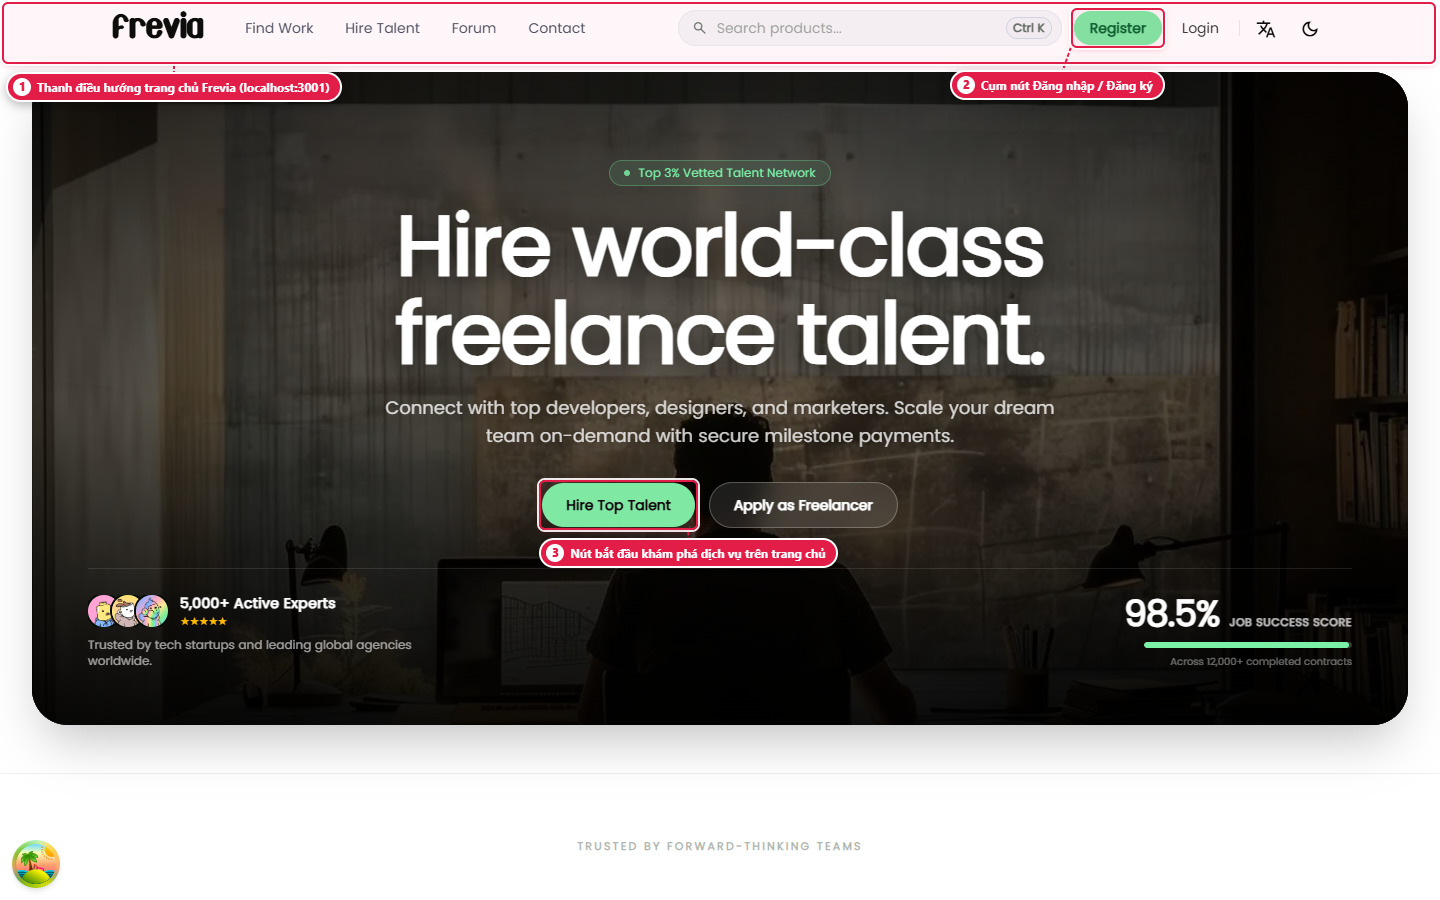
\includegraphics[width=0.90\textwidth]{images/install/a09_verify_web_running.png}
  \caption{Verifying the Next.js web application running at http://localhost:3001}
\end{figure}

\begin{itemize}[leftmargin=1.5em,itemsep=3pt]
  \item \rbadge{1} Open a modern web browser and navigate to \url{http://localhost:3001}. Confirm that the header renders navigation links (\textit{Browse Jobs}, \textit{Freelancers}, \textit{Community}) alongside \textbf{Sign in} and \textbf{Sign up} buttons.
  \item \rbadge{2} Verify that the hero banner renders correctly with the AI search interface, featured skills pills, and call-to-action buttons.
\end{itemize}

\subsubsection{2. Backend RESTful API \& Health Check Verification}

\begin{figure}[H]
  \centering
  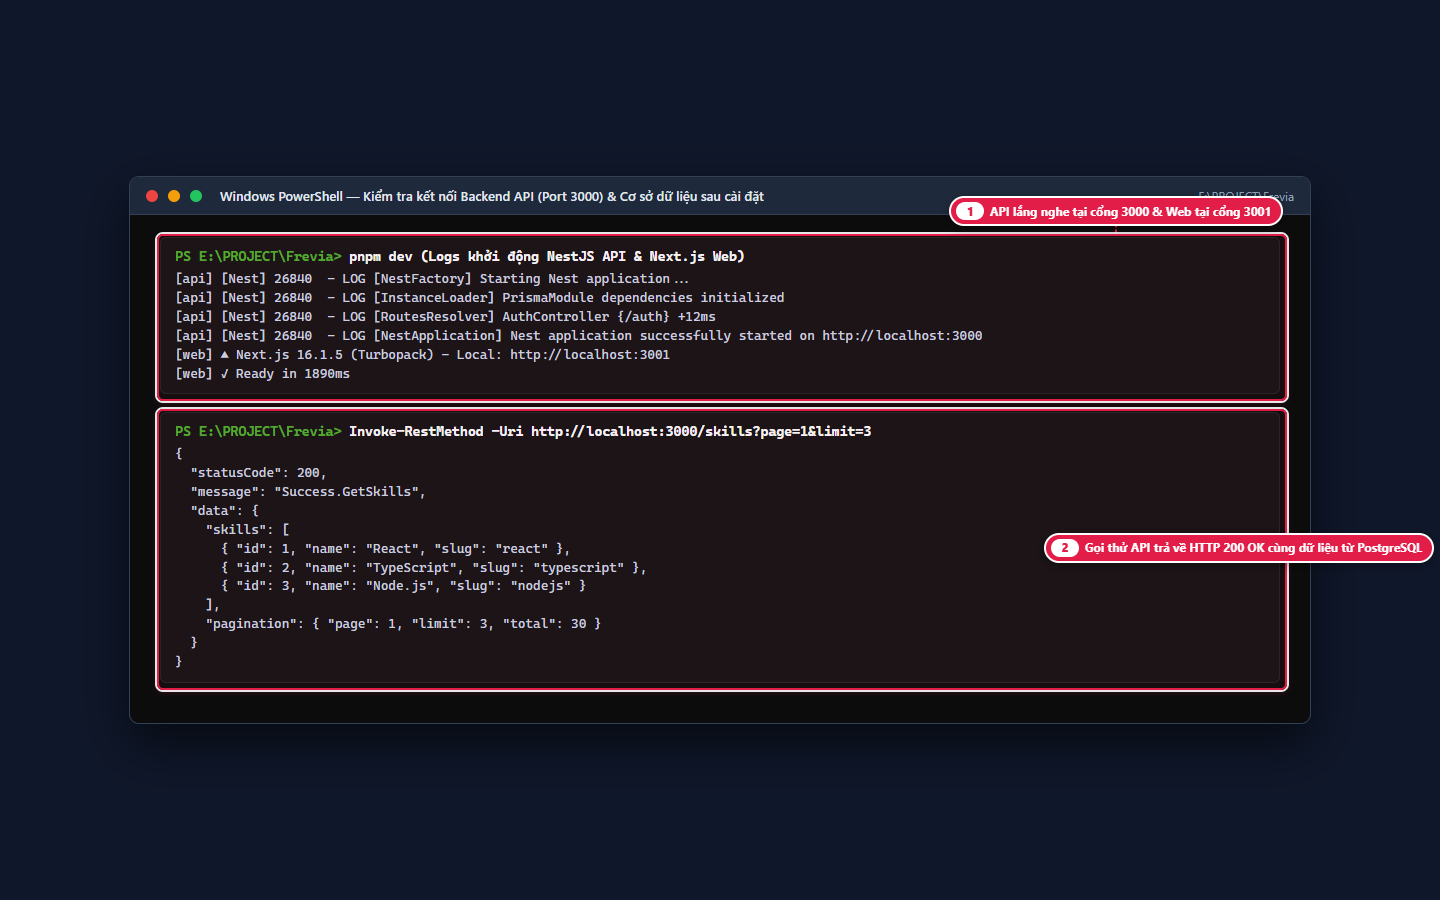
\includegraphics[width=0.90\textwidth]{images/install/a10_verify_api_swagger.png}
  \caption{Verifying Backend RESTful API endpoints and response payloads via HTTP request}
\end{figure}

\begin{itemize}[leftmargin=1.5em,itemsep=3pt]
  \item \rbadge{1} Query the public skills catalog API:
\begin{lstlisting}[frame=single,basicstyle=\footnotesize\ttfamily,backgroundcolor=\color{codebg}]
Invoke-RestMethod -Uri "http://localhost:3000/skills" -Method Get
\end{lstlisting}
  Confirm an \textbf{HTTP 200 OK} status returning a structured JSON response array populated with seed skill records.
  \item \rbadge{2} Test the Redis cache connection:
\begin{lstlisting}[frame=single,basicstyle=\footnotesize\ttfamily,backgroundcolor=\color{codebg}]
docker exec -it frevia-redis redis-cli ping
# Expected output: PONG
\end{lstlisting}
\end{itemize}

\subsubsection{3. Pre-Configured Test Accounts}

The database seeder automatically initializes dedicated accounts across all primary system roles to streamline functional evaluation:

\begin{center}
\renewcommand{\arraystretch}{1.45}
\begin{longtable}{|L{2.8cm}|L{4.2cm}|L{3.2cm}|L{4.2cm}|}
\hline
\rowcolor{hdrfill}\hd{Role} & \hd{Email Address} & \hd{Default Password} & \hd{Assigned Access Scope} \\ \hline
\endhead
\textbf{Administrator} & \texttt{admin@gmail.com} & \texttt{admin123456} & Complete access to \url{http://localhost:3001/admin} (All 275 permissions). \\ \hline
\textbf{Freelancer} & \texttt{freelancer@gmail.com} & \texttt{freelancer123456} & Profile management, AI CV analysis, proposals, contract milestones, payouts. \\ \hline
\textbf{Client} & \texttt{client@gmail.com} & \texttt{client123456} & Job posting, candidate review, milestone funding, escrow deposits. \\ \hline
\textbf{Expert} & \texttt{expert@gmail.com} & \texttt{expert123456} & Expert profile workspace (\texttt{/expert/profile}), revision submissions. \\ \hline
\end{longtable}
\end{center}
